\chapter{Standardization and Normalisation}

\label{ch:standardization-and-normalization}
\index{standardization and normalization|(}

Data \emph{standardization} and \emph{normalisation} are crucial data preprocessing stages in order to prepare the data for machine learning or data mining purposes\footnote{\url{http://www.dataminingblog.com/standardization-vs-normalization/}}.  Standardization is related to the act of centre-reducing the data and a common measure used is the \emph{standard deviation}\index{standardization and normalization!standard deviation}.  This is used in machine learning algorithms such as SVM \index{SVM} or regression \index{regression} problems.  On the other hand, normalisation is a process concerned with scaling or mapping the data in order to make it easier to work with \citep{patro2015normalization}.  Normalisation is useful in almost every machine learning algorithm (such as regression, kNN, neural networks) since it essentially cleans the data.  In this section we shall see a few standardization and normalisation techniques that are related to machine learning.



\section{Min-Max Normalisation}
Min-Max \index{standardization and normalization!Min-Max}is a linear normalisation technique and hence it does not alter the distribution of a data set.  Its goal is to transform the features of a data set to fit within a smaller and more specific range.  Normally this new range is set to $[0,1]$ (see Equation~\ref{eq:sn_min-max}) or $[-1,1]$.  This technique is sometimes called \emph{feature scaling}\index{standardization and normalization!feature scaling}.

\begin{equation}
% there is more than one form for this equation
\label{eq:sn_min-max}
x^{\prime}_{i} = \frac{x_{i} - x_{min}}{x_{max} - x_{min}}
\end{equation}

In equation~\ref{eq:sn_min-max} above, $x^{\prime}_i$ is the normalised value, $x_{i}$ is the unnormalised value and $x_{max}$ and $x_{min}$ are the maximum and minimum values found in dataset $X$ respectively.  

Equation~\ref{eq:sn_min-max-n} is a generic formula for this technique, where the range is specified at two arbitrary points $a$ and $b$:

\begin{equation}
\label{eq:sn_min-max-n}
x^{\prime}_{i} = (x_{max} - x_{min}) \times \frac{x_{i} - x_{min}}{x_{max} - x_{min}} + x_{min}
\end{equation}

 When compared to other normalisation techniques, the Min-Max is very effective whilst being a simple technique to implement \citep{al2006data}.  However, Min-Max is prone\emph{noise} and therefore produce unstable results as it is highly sensitive to \emph{outliers}\index{outliers} \citep{jain2005score}.

\section{Z-score/Zero-Mean Normalisation}
When applying \emph{z-score}\index{standardization and normalization!z-score} to a data set is the same as standardizing it.  Like Min-Max, this is a commonly used technique and it is easy to implement \citep{jain2005score}.  However, the Z-score or Zero-Mean normalisation affects the distribution of a data set such that it becomes \emph{normally distributed}\index{standardization and normalization!normally distributed}.  Figure \ref{fig:sn_normal-dist} \footnote{\url{https://www.kaggle.com/rtatman/data-cleaning-challenge-scale-and-normalize-data}} shows a plot of a normal distribution, also known as the \emph{Gaussian distribution}\index{standardization and normalization!Gaussian distribution}, compared with the original data (before transformation).

\begin{figure}
	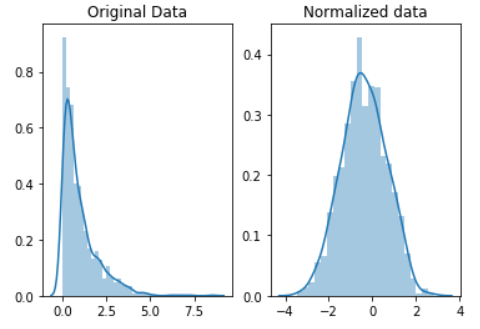
\includegraphics{standardization_and_normalisation/normal-dist.png}
	\caption{Normal Distribution example - notice the "bell curve" of the normalised data}
	\label{fig:sn_normal-dist}
\end{figure}

Equation~\ref{eq:sn_z-score} below shows how z-score is computed by normalising value $v_{i}$ of attribute $A$ to $v^{\prime}_{i}$:

\begin{equation}
\label{eq:sn_z-score}
v^{\prime}_{i} = \frac{v_{i} - \bar{A}}{\sigma_{A}}
\end{equation}

where $\bar{A}$ is the arithmetic mean and $\sigma_{A}$ is the standard deviation of attribute $A$.  When the minimum and maximum of attribute $A$ are unknown, this method is very useful and therefore preferred over Min-Max \citep{han2011data}.  This method is also highly applicable and effective for clustering algorithms such as \emph{K-means clustering}\index{standardization and normalization!K-means clustering} \citep{mohamad2013standardization} \citep{cheadle2003analysis}.

\section{Median Normalisation}
The Median normalisation technique works by calculating the \emph{median}\index{standardization and normalization!median} of a sample from a data set, then each element in the sample is divided by the median (see equation~\ref{eq:sn_median}).  This procedure repeated for every sample $s$ in a data set \citep{jayalakshmi2011statistical}.  

\begin{equation}
\label{eq:sn_median}
x^{\prime}_{i} = \frac{x_{i}}{median(s)}
\end{equation}

Equation~\ref{eq:sn_median-sub} is another way how Median normalisation is formulated, by subtracting the median from every element in sample $s$:

\begin{equation}
\label{eq:sn_median-sub}
x^{\prime}_{i} = x_{i} - median(s)
\end{equation}

For ~\ref{eq:sn_median} and  ~\ref{eq:sn_median-sub} $x_{i}$ is the unnormalised element in sample $s$.  Note that this technique known as an intra-slide normalisation because it works with whole arrays/samples of data.  Although this technique does not guarantee high accuracy, it is quite robust since it is much less sensitive to noise than Min-Max or Z-score \citep{jain2005score}.

\section{Sigmoid Normalisation}
The \emph{Sigmoid function}\index{standardization and normalization!Sigmoid function} can be used as a normalisation technique to scale values, usually between -1 and 1.  There are various forms of non-linear Sigmoid functions.  One example is the $tan$ Sigmoid function (refer to figure~\ref{fig:sn_tag-sig})which tends to speed up the normalisation process \citep{jayalakshmi2011statistical}.

\begin{figure}
	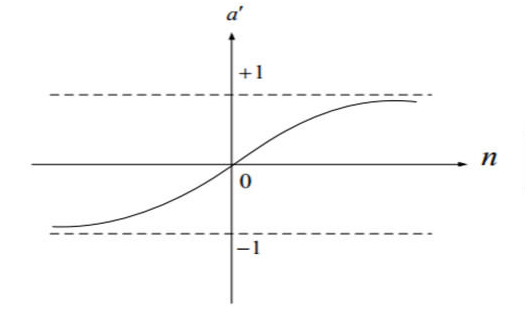
\includegraphics{standardization_and_normalisation/tan-sig.png}
	\caption{$Tan$ Sigmoid Function which can be used as a normalisation technique}
	\label{fig:sn_tag-sig}
\end{figure}

~\ref{eq:sn_tan-sig}is the equation of the $tan$ Sigmoid function:

\begin{equation}
\label{eq:sn_tan-sig}
x^{\prime}_{i} = \frac{e^{x} - e^{-x}}{e^{x} + e^{-x}}
\end{equation}

This normalisation technique is somewhat similar to the Min-Max method since it scales values to a specific range.  However, Sigmoid normalisation is more robust and shows greater efficiency \citep{jain2005score}.  Moreover, there is a more complex form of this technique which is the Double Sigmoid function \citep{cappelli2000combining}.

\section{Batch Normalisation}
\emph{Batch-norm}\index{standardization and normalization!Batch-norm} is a normalisation technique specifically developed for enhancing \emph{neural network}\index{standardization and normalization!neural network} training.  Before this technique was developed, neural networks were only normalised at the input layer only.  The problem with this was that if instability arises in one of the intermediate layers, then the layer would need to readapt to a new distribution thus slowing down the whole process.  This problem is known as \emph{internal covariate shift}\index{internal covariate shift} \citep{ioffe2015batch}.  Batch normalisation solved the problem by adding normalisation at each layer in the network.  Normalisation is done for every input neuron (one batch per neuron) found in the layer (see also figure~\ref{fig:sn_neural}).

\begin{figure}
	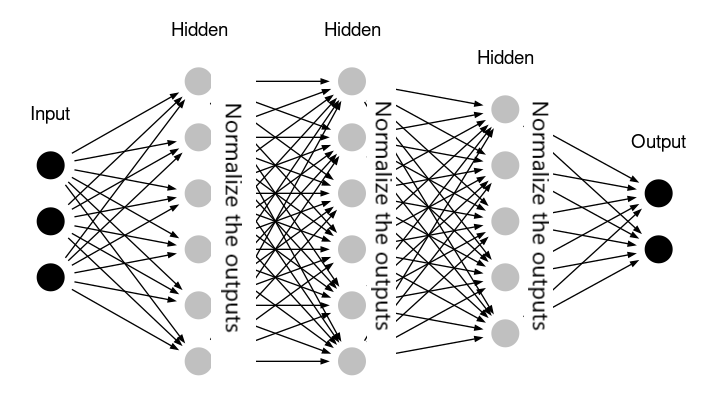
\includegraphics{standardization_and_normalisation/neural-network.png}
	\caption{Neural network with applied batch normalisation \url{https://mc.ai/batch-normalization-speed-up-neural-network-training/}}
	\label{fig:sn_neural}
\end{figure} 

\section{Conclusion}
From these few standardization and normalisation techniques, we have seen the importance to choose the right technique for the right data set (it is important to find out what kind of problem the data set is presenting - for example a regression problem, classification problem, a time-series, text mining and so on).  Some important features that a technique should have are: that it improves accuracy, reduces the training time, simplify the data and robustness to noise.

\index{standardization and normalization|)}
